% !TEX root = main.tex

\section{降维与度量学习}
线性降维方法:对原始高维空间进行线性变换。
给定$d$维空间中的样本$X=(\vx_1,\vx_2,\ldots,\vx_m)\in\rr^{d\times m}$,
变换后得到$d'\leq d$维空间中的样本$Z=W^\T X$,
其中$W\in\rr^{d\times d'}$是变换矩阵,$Z\in\rr^{d'\times m}$是样本在新空间中的表达。

\subsection{k近邻学习}
k近邻(k-nearest neighbor, kNN)是常用的监督学习方法。
给定测试样本,基于某种距离度量找出训练集中与其最为靠近的$k$个训练样本,然后基于这$k$个邻居的信息进行预测。
在分类任务中可以采用投票法,在回归任务中可以采用平均法。

kNN是懒惰学习(lazy learning)的著名代表,在训练阶段仅仅将样本保存起来,训练时间开销为0,待收到测试样本才进行处理。
\begin{figure}[H]
\centering
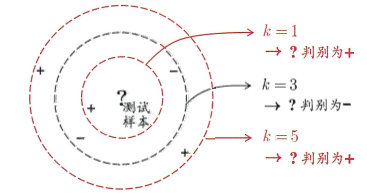
\includegraphics[width=0.4\linewidth]{fig/kNN.png}
\end{figure}

\subsection{主成分分析}
主成分分析(Principle Component Analysis, PCA)希望找到这样的超平面具有这样的性质:
\begin{itemize}
	\item 最近重构性:样本点到这个超平面的距离都足够近,对样本中心化$\sum_i\vx_i=\vzero$,再假定投影变换后得到的新坐标系为$\{\vw_1,\vw_2,\ldots,\vw_d\}$,其中$\vw_i$是标准正交基向量
	\[\norm{\vw_i}_2=1,\vw_i^\T\vw_j=0\;(i\ne j)\]
	\item 最大可分性:样本点在这个超平面上的投影尽可能分开
	\[\begin{aligned}
	\max_{W} &\qquad \optr(W^\T XX^\T W)\\
	\text{s.t.} &\qquad W^\T W=I
	\end{aligned}\]
\end{itemize}

算法流程如下:输入样本集$D=\{\vx_i\}_{i=1}^m$和低维空间维数$d'$
\begin{enumerate}
	\item 对所有样本进行中心化:$\vx_i\gets \vx_i-\frac{1}{m}\sum_{i=1}^m\vx_i$
	\item 计算样本的协方差矩阵$XX^\T$
	\item 对协方差矩阵$XX^\T$做特征值分解
	\item 取最大的$d'$个特征值所对应的特征向量$\vw_1,\vw_2,\ldots,\vw_{d'}$
	\item 输出投影矩阵$W=(\vw_1,\vw_2,\ldots,\vw_{d'})$
\end{enumerate}

降维虽然会导致信息损失,但一方面舍弃这些信息后能使样本的采样密度增大,另一方面当数据收到噪声影响时,最小的特征值所对应的特征向量往往与噪声有关,舍弃可以起到去噪效果。